% Title: Monoids. What, how and why?
% Titulo: Monoides. Que, Como e Por Que?

% Abstract:
% We will learn about Monoids, a concept invented (discovered?) by mathematicians
% that we can leverage to great value in our code and designs.

% The talk is structured in two sessions, in this first one (5/29) we'll learn what
% Monoids are, go through many examples, and write code that creates and uses Monoids. In
% the second session (June maybe?) we will see how we can use Monoids to guide software design.

% Despite the weird name, Monoids are easy to understand, and once you do, you'll
% start finding them everywhere. More importantly, after a little practice
% you'll gain intuition and you'll be able to integrate Monoids in your code and
% designs, obtaining more abstract and reusable results.

% Requirements:
% This is an intermediate level talk. No knowledge of math or functional
% programming is required. I'll assume you can understand simple Scala code.
% In particular, if you don't know what implicit parameters are, spend 10 minutes
% learning about them. You don't need to understand the details of implicit search
% mechanisms or anything like that.


% Resumo:
% Vamos aprender sobre Monoids, um conceito inventado (ou descoberto?) pelos
% matematicos, que nos podemos aproveitar com grandes resultados no nosso codigo e desenhos.

% A palestra esta estruturada em duas sessoes, na primeira (29/05) vamos aprender o
% que sao os Monoids, ver muitos exemplos e escrever codigo que cria e usa
% Monoids. Na segunda sessao (data a confirmar) vamos ver como podemos usar os
% Monoids para guiar o desenho de software.

% Apesar de seu nome estranho, os Monoids sao faceis de entender, e uma vez que os
% entenda, voce vai acha-los em todo lugar. Ainda mais importante, com um
% pouco de pratica, voce vai aprimorar sua intuicao e sera capaz de integrar Monoids no seu
% codigo e desenhos, consiguindo resultados mais abstratos e reusaveis.

% Requerimentos:
% Essa e uma palestra de nivel intermediario. Nao precisa conhecimentos de
% matematica ou programacao funcional. Todos os exemplos serao em Scala, voce devera
% conhecer a linguagem para entende-los. Particularmente, se voce nao sabe o que sao os parametros
% implicitos, gaste 10 minutos aprendedo-os. Nao precisa saber os detalhes dos
% mecanismos de busca de implicitos.

% https://www.theguardian.com/info/developer-blog/2016/dec/22/parental-advisory-implicit-content
% https://docs.scala-lang.org/tutorials/FAQ/context-bounds.html

% Bio:

% Depois de quase uma década trabalhando em linguagens imperativas, Sebastian
% abraçou a programação funcional e nunca mais olhou para atrás. Nos últimos oito anos
% ele tem trabalhado nas áreas de data science, infraestrutura de Big Data e
% enterprise software, em linguagens como Scala, Haskell e Clojure. Cuidado!
% O Sebastian vai tentar trazer você para o mundo da programação funcional.


\documentclass{beamer}
\usepackage[english]{babel}
\usepackage[utf8]{inputenc}
\usepackage[T1]{fontenc}
\usepackage{pgfpages}
\usepackage{listings}
\usepackage{color}
\usepackage{ulem} % for \sout
\usepackage{tikz}
\usepackage{amsmath}


\mode<presentation>
{
  \usetheme{Madrid}      % or try Darmstadt, Madrid, Warsaw, ...
  \usecolortheme{default} % or try albatross, beaver, crane, ...
  \usefonttheme{default}  % or try serif, structurebold, ...
  \useoutertheme{default}
  \setbeamertemplate{navigation symbols}{}
  \setbeamertemplate{caption}[numbered]

  % \AtBeginSubsection[]
  % {
  %   \begin{frame}<beamer>\frametitle{OUTLINE}
  %     \tableofcontents[currentsection,currentsubsection]
  %   \end{frame}
  % }

}

\pgfdeclareimage[height=0.5cm]{assoc-logo}{assoc.png}
\logo{\pgfuseimage{assoc-logo}}

%\setbeameroption{show notes on second screen}
%\setbeameroption{show only notes}

\setbeamerfont{note page}{size=\tiny}
\setbeamertemplate{note page}[plain]




\title[Monoids]{MONOIDS}
\subtitle{\textit{What}, \textit{How} and \textit{Why}}
\author{Sebastian Galkin}
\institute[@paraseba]{\texttt{@paraseba} \\ \texttt{paraseba@gmail.com}}
\date[Scaladores]{Scaladores - May 2018}
\subject{Talks}

\begin{document}
\lstset{
  language=Scala,
  basicstyle={\small\ttfamily},
  keywordstyle={\usebeamercolor{example text}\color{fg}},
  commentstyle={\usebeamercolor{palette sidebar tertiary}\color{fg!170!}\itshape},
  columns=fullflexible,
  escapechar=~,
  showlines=false,
}


\begin{frame}
  \titlepage
\end{frame}

% Uncomment these lines for an automatically generated outline.
\begin{frame} \frametitle{OUTLINE}
  \begin{columns}[c]
    \column{0.6\textwidth}
      \tableofcontents
    \column{0.4\textwidth}
      \rotatebox{45}{\Large \usebeamercolor[fg]{structure}{\texttt{There will be quizzes}}}
  \end{columns}
  \begin{block}{}
    \centering
    \Large \textbf{Ask questions as we go!}
  \end{block}

  \note{
    Hoje vamos falar sobre Monoides. Depois de uma breve introducao
    sobre abstracao, vou mostrar que eh um monoide, e um monte de
    exemplos de monoides interesantes. Finalmente vamos ver varios
    casos onde podemos usar monoides para melhorar nosso codigo
    e para resolver problemas concretos dificis.

    Para manter voces acordados, e ter certeca que estao entendendo,
    vou fazer perguntas que completam o material.

    Podem me interromper se tever duvidas, ou nao entender. Mesmo se o
    que nao entender for o sotaque, me interrompe e com uma mistura de
    portugues, espanhol e ingles vamos nos entender.
  }

\end{frame}


\begin{frame} \frametitle{ABOUT ME}
  {\LARGE Sebastian Galkin}

  \begin{itemize}
  \item \alert{Functional Programming} for a while.
  \item Mostly big data and enterprise.
  \item People are still scared of FP.
  \item You or your team want to learn FP?
  \color{blue}\texttt{paraseba@gmail.com}
  \end{itemize}

  \note {
    Um pouco acerca de mim: faco programacao funcional exclusivamente
    a ums 8 anos. Scala, Haskell, Clojure e outros. Trabalho em data
    science e infrastrutura para big data, mas com alguns periodos de
    software para enterprise. Adoro FP, me faiz sentir inteligente, me
    diverte, me desafia. Nao imagino como seria voltar para a programacao
    imperativa.

    Um problema da FP eh que da medo. Muitas palavras em latim, muitos
    matematicos, um pouco de soberbia... Precisamos mudar isso. FP nao
    eh dificil, so eh diferente. Nao precisa ser matematico, nem genio,
    so ter vontade.

    Se voce quer aprender, ou se voce quer que seu teame aprenda FP? me
    contata. Vamos conversar.
  }
\end{frame}

\section{Monoids in Code}
\subsection{Abstraction}

\begin{frame} \frametitle{WHAT IS ABSTRACTION?}
  \begin{quote}
\textbf{Abstraction} is the process of extracting the underlying \alert{essence} of a concept,
removing any \alert{dependence} on real world objects, and \alert{generalizing} it so that it
has \alert{wider applications.}\\[2ex] \rightline
  {{\rm --- Wikipedia, \href{https://en.wikipedia.org/wiki/Abstraction_(mathematics)}{\underline{Abstraction (mathematics)}}}}
  \end{quote}

  \note {
    Eu peguei essa cita da pagina da wikipedia dedicada a abstracao em
    matematica. Pega um tempo para ler [esperar 15 segundos].

    Se nao chegou a ler, olha so as partes em vermelho: esencia do conceito,
    dependencias, generalizar, reusar. Sao as mesmas palavras que usamos para
    descreber o que chamamos software de qualidade! Lembre que tirei isso de uma
    pagina que fala de matematica!

    Casualidade? Nao acho.

    Na verdade, o conceito de abstracao que temos na industria de software esta
    muito pouco desenvolvido. A maioria das pessoas quando pensa em abstracao
    pensa em indirecao, ou evitar repeticao de codigo. Mas abstracao nao tem
    nada a ver com isso! Mas essa eh uma outra palestra.
  }
\end{frame}

% \begin{frame} \frametitle{YOU CALL THIS ABSTRACTION?}
%   \begin{quote}
%     I wouldn't really think of abstraction as a mathematical concept. \\[1ex] \rightline
%   {{\rm --- Fishtoaster,
%       \href{https://softwareengineering.stackexchange.com/questions/16070/what-is-abstraction}{\underline{SE Stack Exchange}}}}
%   \end{quote}

%   \begin{quote}
%     A programming abstraction is a simplified model of a problem. \\[1ex] \rightline
%   {{\rm --- C. Ross,
%       \href{https://softwareengineering.stackexchange.com/questions/16070/what-is-abstraction}{\underline{SE Stack Exchange}}}}
%   \end{quote}

%   \note {
%     Vamos ver o que pensa o pessoal da ingeniaria de software sobre abstracao.
%     [esperar 15 segundos]

%     ``Abstracao nao eh um conceito matematico''???

%     ``simplified model of a problem''???

%   }

%   \pause

%   \begin{block}{These are not abstraction}
%   \begin{itemize}
%     \item Indirection.
%     \item Inheritance.
%     \item Factoring out common code to a function.
%     \item Passing to functions only what they need.
%   \end{itemize}
%   \end{block}

%   Really, how abstract is your code?

%   \begin{center}
%     \LARGE
%     \bfseries
%   We suck at abstraction!
%   \end{center}
% \end{frame}

\begin{frame} \frametitle{STANDING ON THE SHOULDERS OF GIANTS}
  Mathematicians are the \alert{masters of abstraction.}
  \begin{itemize}
  \item Maximize generality.
  \item Maximize simplicity (elegance)
  \item Analogies and analogies between analogies.
  \item Reusing whole theories.
  \item Finding ``the right'' level of abstraction.
  \end{itemize}

  \pause

  \begin{block}
    \centering \Large \bfseries
  This is what they have been doing for centuries.
  \end{block}

  \begin{block}{}
  copy steal copy steal copy steal
  copy steal copy steal copy steal
  copy steal copy steal copy steal
  copy steal copy steal copy steal
  copy steal copy steal copy steal
  copy steal copy steal copy steal
  copy steal copy steal copy steal
  \end{block}

  \note {

    Na verdade os maiores expertos em abstracao sao os matematicos. Eles, por
    exemplo, consiguem ``reusar'' nao so teoremas, mas teorias completas! Quando foi
    a ultima vez que voce reusou uma coisa tao simples como um mecanismo de signup?

    Os caras sao incansavels na hora de generalizar os resultados, e o mais
    importante, sabem achar o nivel certo de abstracao para cada tarefa.
    Uma das caracteristicas que mais valore em um desenvolvedor e se ele percebe
    quando o nivel de abstracao esta errado.

    Uma das caracteristicas fundamentales da matematica eh o que eles chaman de
    elegancia, que eh muito similar ao que a gente chama de elegancia no codigo.

    \hrulefill

    Em definitiva, os matematicos arrasam em abstracao ha seculos! Precisamos
    aprender e imitar.

    E com isso em mente, vamos pegar umo dos exemplos de abstracao inventado
    pelos matematicos [passar pagina], e vamos a ver como podemos usar ele no nosso codigo.
  }

\end{frame}


\subsection{What is a Monoid}

\begin{frame} \frametitle{WHAT IS A MONOID?}
  \begin{block}{Monoid}
    A \alert{set} together with an \alert{associative} \alert{operation}
    and an \alert{identity} element.
  \end{block}

  \begin{block}{Components - A Triplet \((A, \bullet, u)\)}
  \begin{itemize}
    \item A [carrier] set (\(A\))
    \item A binary operation (\(\bullet\))
    \item An element of the set \(u\)
  \end{itemize}
  We sometimes say ``\(A\) \emph{has} a Monoid''.
  \end{block}


  \begin{block}{Laws (\(a,b,c \in A\))}

  \begin{description}[Commutativity:]
    \item[Closure:] \(a \bullet b\) is an element of \(A\)
    \item[Associativity:] \((a \bullet b) \bullet c = a \bullet (b \bullet c)\)
    \item[Identity:] \(u \bullet a = a \bullet u \ = a\)
    \item[\sout{Commutativity:}] \(a \bullet b \neq b \bullet a\)
  \end{description}
  \end{block}

  \note {

    O monoide eh um conceito muito simples na verdade. Os  matematicos chamam a
    este tipo de conceito uma estrutura algebraica, mas no caso do monoide eh
    simplesmente uma generalizacao de
    operacoes algebraicas como a soma. Vamos ver
    em mais detalhe:

    \hrulefill

    Para apresentar um Monoide em matematica voce precisa dar tres coisas:

    A primeria eh um conjunto, que pode estar formado por cualquer numero e
    tipo de elementos. Por exemplo, o conjunto dos numeros positivos, ou o
    conjunto dos temes de futbol, ou o conjunto dos cabalos com cabeca de homem
    (que eh o conjunto vazio.). Cuando falamos em software, esse conjunto vai se
    convertir em um tipo, vamos pensar um tipo como o conjunto de todos os
    valores possivels desse tipo. Boolean por exemplo, eh um conjunto com dois
    elementos, true e false.

    A segunda coisa que voce precisa apresentar para ter um monoide eh uma
    operacao binaria em esse conjunto, que chamamos com esse simbolo de bolinha.
    Ou seja uma operacao que recebe dois
    elementos do conjunto e devolve um outro elemento desse mesmo conjunto. Se
    continuamos com o essemplo do conjunto de numeros positivos, a soma, recebe
    dois numeros positivos e devolve outro numero positivo.

    Finalmente, o tercer componente, voce precisa escolher um elemento do conjunto
    que vamos chamar \(u\).

    Entao, um monoide tem treis componentes: um conjunto, uma operacao de dois
    argumentos e um elemento ``especial'' chamado unidad, ou identidad, ou zero

    \hrulefill

    Mas para que essas 3 coisas realmente formem um monoide, eh precisso
    elas  cumplir com certas reglas ou leis. Se voce tem os treis componentes
    mas eles nao cumplem as leis, voce nao tem um monoide, tem uma porcaria que
    se usar como monoide vai dar problema.

    A primeira lei ja falamos: a operacao bolinha tem que dar como resultado um
    elemento do set do monoide, nao pode dar uma coisa por fora. No exemplo do conjunto
    de numeros positivos, a resta nao funcionaria como operacao, porque a resta
    de dois numeros positivos, pode dar um numero negativo, que fica fora do conjunto.

    A segunda lei: a operacao bolinha precisa ser asociativa, isso significa que
    nao importa como voce coloca os parentesis, obtem o mesmo resultado. A soma
    por exemplo eh uma operacao asociativa, sumar 1 e 2, e ao resultado sumar 3,
    eh o mesmo que sumar 1 ao resultado de 2 mais 3.

    Finalmente, a terceira lei do monoide: o elemento ``especial'' que
    escolhemos, \(u\), tem que ser o neutro ou identidade da operacao que
    escolhimos. Ou seja, se o combino com qualquer outro elemento do conjunto usando
    a operacao, nao pode modificar o resultado. No exemplo da soma nos numeros positivos, a identidade
    eh o numero cero, porque se sumo qualquer numero positivo com cero, obtenho
    o mesmo numero, tanto fazendo a + 0 quanto 0 + a.

    Importante, vejam que os monoides nao precisam ser commutativos, isso
    significa que a operacao bolinha nao necesariamente permite intercambiar os
    argumentos. O unico que precisa ser comutativo eh a combinacao com a
    identidade, na terceira lei.

    Como podem ver, o monoide eh super simples, uma operacao asociativa com uma
    identidade. E so. Mas a pesar de ele ser tao simples, eh extremamente
    importante e extremamente conveniente.
  }
\end{frame}


\subsection{Some simple examples}
% \begin{frame}\frametitle{A MONOID IN ``REAL LIFE''}
%   Color addition

%   \begin{columns}[c]
%     \column{0.7\textwidth}
%       \begin{itemize}
%         \item \(A\): the set of all colors
%         \item \(a \bullet b\): color formed adding light of color \(b\) on top
%           of light of color \(a\)
%         \item \(u\): transparent color
%       \end{itemize}

%     \column{0.3\textwidth}

%     \begin{figure}
%         \centering
%         \def\svgwidth{\columnwidth}
%         \input{additive-color.pdf_tex}
%     \end{figure}
%   \end{columns}

%   \begin{block}{Quiz}
%   Is it a commutative monoid?
%   \end{block}

%   \note {
%     O primeiro exemplo que escolhi eh o menos ``matematico'': Um monoide de
%     colores. Vamos la, para definir um monoide precisamos dos tres elementos.

%     Vamos falar que nosso conjunto \(A\) eh o conjunto de todas as cores,
%     incluida a cor transparente.

%     Vamos falar que a operacao do monoide eh ``juntar as cores'', entao, se
%     junto a cor verde com a cor vermelha como mostra na imagem, obtenho a cor amarela.

%     Vamos escolher como \(u\), a identidade, a cor transparente.

%     Entao que nos falta para saber se esse triplete de coisas forma um monoid?
%     Nos falta verificar que se cumplem as leis:

%     Lei 1: posso escoher cualquer duas cores, juntalas e obter outra cor? Sim,
%     sempre vou obter alguma cor, e como o conjunto es o conjunto de \emph{todas}
%     as cores, a lei se cumple.

%     Lei 2: eh a operacao asociativa? Sim (acho, na verdade nao sei nada de
%     cores, mas vamos supor que sim). Isso significa que se junto o vermelho com
%     o verde, e depois adiciono azul, obtenho a mesma cor que se junto vermelho,
%     com verde misturado com azul. Acho que isso eh verdade.

%     Lei 3: escolhimos o transparente como identidade. Precisamos verificar que
%     se misturo trasparente com cualquer cor obtenho a mesma core. Eh verdade,
%     entao pronto, temos um monoid.

%     Eh um monoide commutativo? [Esperar ou responder]
%   }

% \end{frame}

\begin{frame}\frametitle{EXAMPLES OF MONOIDS IN MATH}
  \begin{itemize}
    \item Integers under addition with zero identity.
      \[
      (a + b) + c = a + (b + c) \qquad a + 0 = 0 + a = a
      \]
    \item Integers under multiplication with 1 identity.
      \[
        (a b) c = a (b c) \qquad a \times 1 = 1 \times a = a\]
    \item Subsets of a set under union with empty identity.
      \[
        \mathcal
        (\mathcal{A} \cup \mathcal{B})\cup  \mathcal{C} = \mathcal{A}\cup  (\mathcal{B}\cup  \mathcal{C}) \qquad
        \mathcal{A} \cup \emptyset = \emptyset \cup \mathcal{A} = \mathcal{A}
      \]
    \item Spatial transformations
  \end{itemize}
  \begin{block}{Quiz}
    Integers under division with \(1\) as identity?
  \end{block}
  \note {
    Vamos partir para alguns exemplos bem simples na matematica

    A soma de inteiros usando zero como identidade? Eh um monoide? Vamos ver: se
    sumo dois inteiros sempre obtenho um inteiro. Pronto lei 1. A soma eh uma
    operacao asociativa, nao importa como eu arrumar os parentesis, sempre
    obtenho o mesmo resultado. Pronto lei 2. Sumar cualquer numero com cero, e cero com
    cualquer numero, sempre da o mesmo numero. Pronto lei 3. Entao, eh um
    monoide. De fato, a suma eh uma operacao commutativa: a + b = b + a, entao
    nao so eh um monoide, mas eh um monoide commutativo.

    Do mesmo jeito, os inteiros com a multiplicacao, usando 1 como identidade
    tambem formam um monoide. A demostracao eh igual.

    Conjuntos, usando a uniao como operacao e o conjunto vacio como identidade
    tambem formam um monoide. Cual eh o conjunto desse monoide? O conjunto de
    todos os conjuntos (que eh uma coisa bem paradoxal mas tudo bem...deixa para
    la)

    Tem muitos muitos outros monoides na matematica.

    Que voces acham dos inteiros com divisao? Formam um monoide? (nao, viola as
    3 leis, a mais obvia eh a de closure)
  }
\end{frame}

\subsection{Examples in programming}

\begin{frame}\frametitle{BASIC MONOIDS IN PROGRAMMING}
  \begin{itemize}
    \item<1-> \texttt{Integer} under \texttt{(+)} with \texttt{0}.
    \item<1-> \texttt{Integer} under \texttt{(*)} with \texttt{1}.
    \item\only<1>{\texttt{Double} under \texttt{(+)} with \texttt{0}?}
         \only<2->{\alert{\sout{\texttt{Double} under \texttt{(+)} with \texttt{0}}}
           \hspace{2em}
      \( (0.1+0.2)+0.3 \neq 0.1+(0.2+0.3)\).}
    \item<3-> \texttt{Boolean} under \texttt{||} with \texttt{False}.
    \item<3-> \texttt{Boolean} under \texttt{\&\&} with \texttt{True}.
    \item<3-> \texttt{Set[A]} under \texttt{union}.
  \end{itemize}

  \begin{block}{Quiz}<3->
    \begin{itemize}
    \item What is the identity of the \texttt{Set[A]/union} Monoid?
    \item Is \texttt{Set[A]/union} commutative?
    \end{itemize}
  \end{block}

  \note {
    Vamos a falar de programacao agora. Como falamos antes, agora a conjunto do
    monoid vai a ser um tipo. Entao para identificar um monoide precisamos um
    tipo A, uma funcao que pega dois A e devolve um A, e um valor ou termino de tipo A que sera a identidade.

    Igual que na matematica inteiros com adicao ou multiplicacao formam
    monoides. A operacao eh asociativa, para todo pair de inteiros obtenho um
    outro inteiro sumando ou multiplicando, e tem uma identidade.

    Interesante que ja vemos que o mesmo tipo pode ter mais de um monoid, de
    fato tem muitos monoides interessantes nos inteiros.

    O que voces acham da soma nos numeros de ponto flutuante. Pareceria que
    forma um monoide, mas, viola alguma das leis? [esperar]

    \hrulefill

    Viola a lei de associatividade. A soma de ponto flotante nao eh associativa,
    entao nao temos um monoide.

    \hrulefill

   E tem mais exemplos de monoides. Por exemplo os booleanos com OR e False,
   formam um monoide. Porque a || false eh igual a false || a = a

   Os sets formam um monoide usando a uniao como operacao. Qual eh a identidade?

   Os mapas formam um monoide tambem, na verdade varios, mas por exemplo podemos
   usar o merge como operacao e o mapa vacio como identidade.
  }
  \end{frame}

\begin{frame}[fragile]\frametitle{MODELING MONOIDS IN SCALA}
  If the type \texttt{A} \emph{has} a monoid we need:
  \begin{itemize}
    \item a way to create an \texttt{A} from nothing,
    \item a way to combine two \texttt{A}s.
  \end{itemize}
  \pause

  \begin{block}{}
  \begin{lstlisting}
trait Monoid[A] {
  // The identity
  def zero: A

  // The associative operation
  def append(a: A, b: => A): A
}
  \end{lstlisting}
  \end{block}

  \pause

  We can have more than one Monoid for the same \texttt{A}
  \begin{block}{But wait}
    What happened to the laws?
  \end{block}

  \note {
    Vamos ver agora como escribir monoides em scala, como modelar eles. Que
    vamos precisar? um tipo A, uma funcao que recebe dois A e devolve outro A. E
    uma identidade, que eh un valor de tipo A. Correto? Os treis componentes do monoide.
    Como escrebemos isso em scala?

    \hrulefill

    Bom, podemos usar um trait. O jeito de ler isso seria: para um tipo A, posso
    ter um monoide se eu implementar duas funcoes: uma a funcao sem argumentos que me devolve a
    identidade do monoide (aqui chamamos de zero), e outra que eh a operacao
    binaria do monoide (aqui chamamos de append).

    Nao da muita bola para o fato de que o segundo argumento de append eh
    passado por nome, eh um detalhe opcional, e nao quero me focar nisso agora.

    Correto? parece uma codificacao razoavel do conceito de monoide? Simples neh?

  \hrulefill

    Interessante perceber que com esse trait, podemos ter muitas instancias
    diferentes, que eh o que queriamos verdade? Um inteiro pode ter muitos
    monoides differentes, com differentes identidades e operacoes.

    Mas para asegurar que um objeto que implementa esse trait realmente eh um
    monoide, lembremos que precissamos verificar as leis do monoide. Se eu te
    dou un objecto que extiende esse trait, como voce se sabe que o objeto
    cumple as leis? Bom ... nao sabe. Voce vai a escutar por ai que os sistema
    de tipos do scala nao eh suficientemente poderoso para capturar as leis do
    monoide. E eh isso que significa, os tipos nao garantem que o objeto eh um
    monoid, voce tem que confiar em quem implementou. Fazer o que. Mas sempre,
    vamos ter que verificar manualmente as leis, nao queremos dar para ninguem
    um objeto que parece um monoide mas que nao eh, as consequencias sao
    terrives, e ja vamos falar disso mais para frente.
  }
\end{frame}

\begin{frame}[fragile]\frametitle{OPTIONAL SYNTAX SUGAR}
  \begin{block}{}
  \begin{lstlisting}
import MonoidSyntax._  // assume this in all slides

a |+| b === implicitly[Monoid[A]].append(a,b)  // nicer syntax
  \end{lstlisting}
  \end{block}

  \begin{block}{No need to understand this code}
  \begin{lstlisting}
object Monoid {
  def apply[A:Monoid]: Monoid[A] = implicitly[Monoid[A]]
}

object MonoidSyntax {
  implicit def ToMonoidOps[A:Monoid](v: A) = new MonoidOps[A](v)
  final class MonoidOps[A:Monoid](val self: A) {
    def |+|(other: => A): A = Monoid[A].append(self, other)
  }
}
  \end{lstlisting}
  \end{block}
  \note {
    Uma coisa que vou adicionar agora, so para deixar mais curtos os slides eh
    uma syntaxe optional. Ao embez de ter que ussar o metodo append do trait que
    acabamos de definir, posso usar esse operador de soma com barras de modulo,
    que fica mais curto. Nao precisa entender o codigo, so saibam que se tem um
    monoide que posso achar implicitamente, posso usar o operador soma modulo.
  }
\end{frame}

\begin{frame}[fragile]\frametitle{TWO MONOIDS FOR \texttt{Int}}
  \begin{block}{}
  \begin{lstlisting}
val intAddMon = new Monoid[Int] {
  def zero: Int = 0

  def append(a: Int, b: => Int): Int =
    a + b
}

val mulMon = new Monoid[Int] {
  def zero: Int = 1

  def append(a: Int, b: => Int): Int =
    a * b
}
  \end{lstlisting}
  \end{block}
  Monoids \alert{instances} are first class citizens

  \note {
    Pronto! vamos a escreber uns monoids entao!

    Os dois mais facis que vimos, inteiros com soma e inteiros com multiplicacao.

    Interessante perceber que esses sao monoides, ou seja, cumplem as leis do
    monoid, mesmo que os inteiros fazem overflow quando pasa do numero maximo.
    Pode tentar probar isso em casa.

    Simplesmente preciso cria uma clase anonima, que implemente as duas funcioes
    do trait Monoid.

    Entao, new Monoid[Int], o zero eh o numero zero, e o append eh a soma. E o
    mesmo para a multiplicacao, identidade 1 o append multiplicacao.

    Como voces vem, os monoides sao objetos como cualquer outro, simplemente um
    valor que posso passar a funcioes, colocar em listas, etc.

    Um ponto importante. Lembram das leis dos monoides? Eu escrivi dois monoids,
    mas cade as leis? Como sei que a operacao eh commutativa, como sei que tem
    um neuto ou identidade? A resposta eh que nao sei. Em scala as leis tem que
    ser probadas com papel e lapis, ou com tests, nao posso codificar as leis no
    sistema de tipos. Outras linguagens mais complexas permitem, mas nao vamos
    entrar nisso. O importante, toda vez que escrivir um monoide, verifique as
    leis manualmente, idealmente escriba num comentario se foram dificis de
    probar, e faza tests.

    Pronto, ja sabemos o que eh um monoide, e ja escrebimos os primeiros dois. Facil!
  }
\end{frame}

\begin{frame}[fragile]\frametitle{THE LIST MONOID}
  \begin{block}{A default (?) Monoid for Lists}
  \begin{lstlisting}
implicit def freeMon[A]: Monoid[List[A]] = new Monoid[List[A]] {

  def zero: List[A] = List()

  def append(as: List[A], bs: => List[A]): List[A] =
    as ++ bs
}
  \end{lstlisting}
  \end{block}

  \begin{block}{Quiz}
Is \texttt{freeMon} a commutative monoid?
  \end{block}

  \note {
    Vamos a escreber um monoid mais interesante agora. Se usamos listas de A
    como o tipo do nosso Monoid. Que podemos usar como zero e append? Bom, a
    concatenacao de listas eh asociativa, e a lista vacia concatenada com
    qualquer outra lista, tanto no comeco como no final, deixa a lista igual.
    Entao isso forma um monoide.

    Voces acham que esse eh um monoide commutativo? [esperar]. Nao, claro que
    nao eh a concatenado com b nao eh o mesmo que b concatenado com a.

    Ja temos 3 monoides! (nao sabemos para que serve, mas confia...) Vamos por mais!
  }
\end{frame}

\begin{frame}[fragile]\frametitle{MONOID FOR TUPLES}
  How can we combine two tuples \texttt{(A,B)}:

  {\small \texttt{(4, List('H','e','l','l','o')) |+| (2, List('W','o','r','l','d'))}}

  \pause

  If \texttt{A} and \texttt{B} have Monoids themselves, we can \alert{combine componentwise}.


  \pause

  \begin{block}{}
  \begin{lstlisting}
implicit def pairMon[A: Monoid, B: Monoid] = new Monoid[(A, B)] {
  /* ~\phantom{cit def pairMon[A: Mon}\rotatebox[origin=c]{90}{$\Rsh$}~ syntax sugar for:
     (implicit am: Monoid[A], implicit bm: Monoid[B]) */

  def zero: (A,B) =
    (Monoid[A].zero, Monoid[B].zero)

  def append(a: (A, B), b: => (A, B)): (A,B) =
    (a._1 |+| b._1, a._2 |+| b._2)
}
  \end{lstlisting}
  \end{block}

  \note {
    Podemos criar um monoide para pares? como combinamos dois pares (a,b)? por
    exemplo, te dou dois pares de um inteiro e uma lista. [esperar]

    \hrulefill

    Teriamos que combinar cada componente neh? o 4 com o 8 e a lista hello com a
    lista world. Mas como combinamos esses componentes? Alguma ideia? [esperar]

    Bom, se os componentes tiveram eles mesmos monoids, poderiamos usar o
    monoid para combina-los neh?

    \hrulefill

    Entao vamos la para escriber o metodo append do monoid de pares,
    simplesmente uso o monoide dos elementos. Da para ver? o primeiro mais na
    definicao de append corresponde a o monoid do tipo A, e o segundo mais ao
    monoide do tipo B. Em geral sao codigos diferentes. Em nosso caso, se usamos
    o monoide de suma de inteiros e o monoide de concatenacao de listas, o
    resultado vai ser o par 6 com a lista helloworld

    Quanto ao zero, o mesmo truque, uso o zero do monoid do tipo de cada componente.

    Agora olha a definicao da funcao, estou devolvendo um novo monoid para pares A
    e B, mas isso so vai a funcionar se posso achar monoids para A e para B. Se
    nao tenho esses monoides, nao saberia como combinar as componentes, e o
    codigo nao compila. A syntaxe essa A:Monoid e B: Monoid, eh so syntax sugar
    para parametros implicitos, eh o mesmo que receber dois parametros
    implicitos de tipo Monoid[A] e Monoid[B].
  }
\end{frame}


\begin{frame}[fragile]\frametitle{IS THERE A MONOID FOR FUNCTIONS?}
  It seems hard for arbitrary functions \texttt{A => B}.

  \pause
  But how about \alert{\texttt{A => A}}?

  \pause

  \begin{block}{Functions that take and return the same type}

  \begin{lstlisting}
implicit def endoMon[A] = new Monoid[A => A] {

    def zero: A => A = ~\only<3->{identity}~

    def append(f: A => A, g: => (A => A)): A => A =
      ~\only<3->{g andThen f}~
  }
  \end{lstlisting}
  \end{block}
  \begin{block}<3->{Quiz}
    \begin{itemize}
      \item Is it a commutative Monoid?
      \item Can we do \texttt{(f andThen g)} instead?
    \end{itemize}
  \end{block}

  \note {

    Continuando para coisas mais dificis. Como voces combinariam funcoes de A a B?

    \hrulefill

    Parece dificil, mas e se foram funcoes de A a A. Como podemos combinar duas
    funcoes de A a A e obter outra funcao de A a A?

    \hrulefill

    Bom, posso simplesmente compor as duas funcoes neh? Isso me da uma nova
    funcao que tambem vai de A a A. E qual eh a identidade da composicao de
    funcoes? a funcao identidade justamente. Si compongo cualquer funcao com a
    funcao identidade obtenho a mesma funcao original.

    Entao o codigo fica muito simples: crio um novo monoid onde o zero eh a
    funcao identidade e o append eh a composicao das funcoes. Olhem o tipo de
    append: recebe duas funcoes e devolve uma funcao.

    Certo?

    Voces acham que eh um monoide commutativo esse aqui? [esparar]. Nao, claro
    que nao, por exemplo primeiro somar 1 e depois elevar ao cubo, nao eh o
    mesmo do que primeiro elevar ao cubo e depois sumar 1.
  }
\end{frame}


\begin{frame}[fragile] \frametitle{A DIFFERENT MONOID FOR FUNCTIONS}
  How about \texttt{(A => B)} where \alert{\texttt{B} has a Monoid?}

  \begin{block}{Functions that return a monoidal type}
  \begin{lstlisting}
implicit def monFunMon[A, B:Monoid]: Monoid[A => B] =
  new Monoid[A => B] {

    def zero: A => B =
      _ => Monoid[B].zero

    def append(f: A => B, g: => (A => B)): A => B =
      a => f(a) |+| g(a)
}
  \end{lstlisting}
  \end{block}
  Convince yourself that \texttt{zero} is an identity and that \texttt{append} is associative.

  \note {
    Tem mais um monoide simples que podemos escreber fara funcoes. Acabamos de
    escreber um para funcoes de tipo A => A, mas se a funcao retorna um tipo que
    tem um monoide ele mesmo, similar ao caso dos pares, podemos usar o monoide
    de B para combinar os resultados.

    Vamos la, para implementar a funcao zero, preciso devolver o que? Um valor
    de tipo funcao de A a B. Como posso criar essa funcao do nada? Bom, como eu
    tenho um monoide para B, poso devolver uma funcao que sempre devolve o zero
    de B.

    E para o append? tenho duas funcoes que devolvem um B, as chamo as duas, e
    depois combino os dois B usando a operacao do monoide.

    Agora nao eh tao obvio ver que as leis do monoide se cumplem, mas pensando
    um pouquinho voces podem verificar. Nao esquecam, muito importante verificar
    as leis.
  }
\end{frame}

% \begin{frame}[fragile] \frametitle{OPTION MONOIDS}
%   % \begin{block}{Quiz}
%   %   Would it make sense to try to write an instance of
%   %   \texttt{Monoid[Option]?}
%   % \end{block}

%   % \note {
%   %   Vamos escreber monoide para Option agora. Faiz sentido um Monoid[Option]?
%   %   [esperar]. Por que nao? Porque option nao eh um tipo, eh um construtor de
%   %   tipos! Nao posso devolver uma valor de tipo Option, tem que ser Option de
%   %   alguma  coisa, Option[Int], Option[String], etc.

%   % }

%     There are several ways to combine two \texttt{Option[A]}

%   \begin{block}{Taking the first \texttt{Some}}
%   \begin{lstlisting}
% def firstMon[A]: Monoid[Option[A]] = new Monoid[Option[A]] {

%   def zero: Option[A] = None

%   def append(a: Option[A], b: => Option[A]): Option[A] =
%     a orElse b
% }
%   \end{lstlisting}
%   \end{block}

%   Similarly taking the last \texttt{Some}
%   \begin{block}{Quiz}
%     \begin{itemize}
%     \item What does \texttt{firstMon} do when combining a bunch of \texttt{Options}?
%     \item Is it commutative?
%     \end{itemize}
%   \end{block}

%   \note {
%     Vamos escreber um monoid para Option[A]. Que posso devolver no zero? Tem que
%     ser um option de A. Bom, posso devolver None, sem problema.

%     E como combino dois Option[A] para obter outro Option[A]? Bom, posso ficar
%     com o primeiro que nao seja None. Se a eh um Some, usso a, e se nao uso b.
%     Ou tambem poderia fazer no contrario se quiser.

%     Que voces acham que o monoide esse faiz, se eu combinar um monte de
%     Option[A] usando append? [esperar] vai me devolver o primeiro que esteja
%     definido, que nao seja vazio.

%     Eh commutativo? [esperar]. Nao, se falamos que devolve o primeiro Option que
%     nao eh vazio, o da izquerda, se agora eu chamar com os argumentos no
%     contrario, o resultado em geral sera diferente.
%   }

% \end{frame}


\begin{frame}[fragile] \frametitle{OPTION WRAPPING A MONOIDAL TYPE}
  \begin{block}{Using the wrapped monoid (one of several monoids for \texttt{Option[A]})}
  \begin{lstlisting}
def optionMon[A:Monoid]: Monoid[Option[A]] = new Monoid[Option[A]] {
  def zero: Option[A] = None   // --- weird ---

  def append(a: Option[A], b: => Option[A]): Option[A] =
    (a,b) match {
      case (a, None) => a
      case (None, b) => b
      case (Some(a), Some(b)) => Some(a |+| b)
    }
}
  \end{lstlisting}
  \end{block}

  \begin{block}{Quiz}
    \begin{itemize}
      \item Why is \texttt{zero} weird?
      \item Can we do \texttt{zero = Some(Monoid[A].zero)} instead?
    \end{itemize}
  \end{block}

  \note {
    Tem muitas formas de crear monoids para Option[A], aqui vemos uma que eh
    util, mas na verdade todas as outras tambem sao utis.

    Aqui vamos a usar o mesmo truque que usamos para funcoes. Vamos a pedir que
    o tipo A, de noso monoid de Option[A] tenha um Monoide tambem. Entao, como
    vamos combinar dois Option[A] para obter um outro Option[A]? Como o A tem um
    monoide, podemos usa-lo para a combinacao. Entao, se os Option que
    recebemos sao os dois Some de alguma coisa combinamos essas coisas usando a
    operacao do monoide de A, se temos so um so Some, e o outro e None,
    simplesmente retornamos o que tem informacao.

    E para o zero? Para o zero precisamos devolver None, porque lembramos que
    tem que ser uma identidade do append, e quando o apend recebe um None,
    devolve o outro elemento sem modificar.

    Mas eu marquei ai que a implementacao de zero esta estranha. Por que voces
    acham que esta estranha essa implementacao, mesmo que esteja correta, todas
    as leis se cumplem. [esperar] O segundo ponto do exercicio pode ajuda-los.
    [esperar]. A racao pela qual essa implementacao eh estranha eh porque nao
    usamos o metodo zero do monoide de A. Podemos usa-lo? que acontece se
    devolvemos Some(m.zero)? Nao  podemos, isso violaria a lei de identidade
    porque zero com None daria zero, ao envez de none.

    A solucao de esse problema aparece com uma outra estrutura algebraica, mais
    simples do que o monoid, que se chama semigroup. Um semigroup eh
    simplesmente um monoide sem zero. Mas vamos deixar isso para uma outra vez,
    ou voces podem ler ao respeito.
  }
\end{frame}

\begin{frame} \frametitle{RECAP}
  We have seen:
  \begin{itemize}
    \item Monoid definition (binary assoc operation with identity).
    \item Monoid \texttt{trait} (one type parameter,
      two methods: \texttt{zero, append})
    \item Monoids for:
      \begin{itemize}
      \item Numbers, lists, tuples (if components have Monoids)
      \item \texttt{A => A} and \texttt{A => M} where \texttt{M} has a Monoid
      \item \texttt{Options}
      \item There are many, many more.
      \end{itemize}
  \end{itemize}

  \begin{block}{}
    \centering
    But we haven't seen \alert{why} or \alert{how} to use monoids.
  \end{block}

  \note {
    Recapitulando: ja Vimos o que eh um monoide, ja vimos como modelar um
    monoide em scala, usando um trait com os dois metodos zero e append. E ja
    vimos varios monoides implementados, para numeros, listas, pares, funciones, etc

    Mas o que nao vimos eh como usar os monoides, para que eles servem o como
    usal-os. O resto da palestra vai ser exemplos de como usar monoides em
    codigo, para resolver problemas. Vamos la!
  }
\end{frame}

\subsection{Usage}
\begin{frame}[fragile] \frametitle{SIMPLE USAGE EXAMPLES}
  \framesubtitle{\texttt{mconcat}}

  \begin{block}{A useful little function}
  \begin{lstlisting}
// mconcat( List(a1, a2, a3) ) === a1 |+| a2 |+| a3
def mconcat[A:Monoid](as: Traversable[A]): A =
  as.foldLeft(Monoid[A].zero)(_ |+| _)~\pause~

def sum(xs: Traversable[Int]): Int = ~\alert{mconcat}~(xs)(intAddMon)

def concat[A](xs: Traversable[List[A]]): List[A] =
  ~\alert{mconcat}~(xs)(freeMon) // or get the Monoid implicitly

def sumO[A](xs: Traversable[Option[Int]]): Int =
  ~\alert{mconcat}~(xs)(optionMon(intAddMon))

sumO(Vector()) = Nothing
sumO(Vector(Some(5), Some(1), None, Some(3))) === Some(9)
  \end{lstlisting}
  \end{block}

% def ~\alert{xyz}~[A](xs: Traversable[Option[A]]): Option[A] =
%   mconcat(xs)(firstMon)

  % \begin{block}<3->{Quiz}
  %   What does \texttt{xyz} do?
  % \end{block}

  \note {
    O primeiro que vamos fazer eh escribir uma funcao muito util, chamada de
    mconcat. Essa funcao recebe uma lista ou sequencia de elementos, e usa um
    monoide implicito para comprimir, o juntar,o colapsar todos eles em um elemento so.
    Entao recebe uma lista de A e develve um unico A.

    Como implementamos mconcat? Simplesmente temos que por um |+| entre cada umo
    dos elementos da lista. E isso eh essatamente o que os folds fazem. Nesse
    caso estou implementando com foldLeft, mas foldRight daria o mesmo resultado.
    A unica diferenca entre usar foldLeft e foldRight seria como os parentesis
    sao colocados, e se o zero do monoide se combina com o primeiro o ultimo
    elemento, mas ja sabemos que essas duas coisas, para um monoide, e so para
    um monoide, nao importam.

    \hrulefill

    Agora que temos a funcao mconcat, vemos que ela eh muito util, nos permite
    implementar funcoes bem utis como essas 3 aqui. Podemos somar uma lista de
    inteiros, simplesmente passando um monoide de soma que ja vimos. Podemos
    concatenar listas, pasando o monoide de listas. E podemos hacer coisas mais
    interessantes como sumo Options[Int], ignorando os que estajam vazios.
    Podem ver o monoid que estou usando em sumO, eh o monoide de Option
    que vimos, que precisa de um outro monoid para combinar. Aqui tambem podemos
    ver aquela coisa estranha que tinhamos visto nesse monoid, quando a lista
    esta vazia a funcao devolve None, ao en vez de cero. Porque o zero do monoid
    de Option era None.
  }

\end{frame}

\begin{frame}[fragile] \frametitle{SIMPLE USAGE EXAMPLES}
  \framesubtitle{Functional MapReduce}
  \begin{block}{Super useful: \texttt{foldMap}}
  \begin{lstlisting}
def foldMap[A, M:Monoid](as: Traversable[A], f: A => M): M =
  //  === mconcat(as.map(f))

  as.foldLeft(Monoid[M].zero) { (res,x) => res |+| f(x) }
  \end{lstlisting}
  \end{block}

  \texttt{f} acts as the mapping phase in a MapReduce, the monoidal
  operation is the reduction step.

  \begin{block}{}
  \begin{lstlisting}
def filter[A](as: List[A], f: A => Boolean): List[A] =
  foldMap(as, (a:A) =>
    if (f(a)) List(a)
    else List())(freeMon)
  \end{lstlisting}
  \end{block}

  \note {
    Mais uma funcao muito util que podemos definir eh foldMap, essa funcao
    aparece muito, eh super util, e se comporta mais ou menos como um mini
    MapReduce. foldMap procesa uma sequencia de As e recebe uma funcao que sabe
    convertir um A em um outro tipo cualquer M, mas com a condicao de que o M
    precisa ter um Monoid

    Para implementa-la, podemos fazer como no comentario, simplesmente mapear
    com a funcao f, e depois chamar mconcat para colapsar todos os M com o
    monoide. Isso funciona sem problema mais faze duas passadas pela sequencia,
    entoa tem uma outra implementacao tambem simples usando foldLeft ou
    foldRight. Mas quando pensar em foldMap, convein imaginar ela como map,
    seguido de mconcat: map seguido de reduce.

    Tendo foldMap podemos implementar uma grande lista de funcoes, em
    particular, tendo foldMap podemos implementar foldLeft, foldRight etc. Como
    exemplo aqui vemos a funcao filter implementada como um foldMap. o que
    fazemos eh convirtir cada elemento da lista em uma lista, e depois deixar
    que o monoide de listas (que so concatena) junte as listinhas de um
    elemento. A lista que devolvemos eh uma lista que esta vazia para os
    elementos que nao cumplem o predicado, e contem o elemento se o predicado se satisface.
  }
\end{frame}


\begin{frame}[fragile] \frametitle{COMPOSING MONOIDS}
  \framesubtitle{Combining predicates}
  \begin{block}{Boolean has Monoids}
  \begin{lstlisting}
  implicit val allMonoid: Monoid[Boolean] = new Monoid[Boolean] {
    def zero: Boolean = true
    def append(a: Boolean, b: => Boolean): Boolean = a && b
  }
  \end{lstlisting}
  \end{block}

    Then predicates have Monoids remember?

    \texttt{def monFunMon[A, B:Monoid]: Monoid[A => B]}

  \begin{visibleenv}<2->
  \begin{block}{}
  \begin{lstlisting}
  val numbers = (1 to 100).filter(   // type annotations needed
    (_ % 2 == 0) |+| (_ >= 10) |+| (_ < 20)
  )

  === Vector(10, 12, 14, 16, 18)
  \end{lstlisting}
  \end{block}
  \end{visibleenv}
  \note {

    Uma das grandes ventagems dos monoides eh que eles se componem muito bem.
    Vamos ver 2 exemplos do que significa ``componer''.

    Nesse primeiro exemplo vamos a escribir um Monoide para booleanos. Podemos
    ver que o unico que o monoide faz eh faver o AND dos dois booleanos, e o
    zero eh claro que eh true, porque true AND x = x para todo x. Entao muito
    bem, AND eh uma operacao asociativa, true eh a identidade, entao boolean tem um monoide.

    Mas se voces recordarem, tinhamos escribido um monoide para funcoes que
    devolvem um monoide. Lembra? combinaba funcoes chamando as duas funcoes e
    combinando os resultados com o monoide. Isso significa que se temos um
    monoide para booleanos, tambem temos um monoides para funcoes que devolvem
    booleanos, ou seja, para predicados.

    \hrulefill

    E que podemos fazer com esse Monoide? bom, por exemplo podemos combinar
    predicados para chamar a filter. Esses 3 predicados estao sendo combinados
    com AND pelo monoide, isso vai devolver so os elementos que cumplem os treis
    predicados.

    Nos nao escrebemos um monoide para predicados, mas esse monoide veio de
    graca, porque escrebemos monoides para funcoes e para booleanos, e os
    monoides se componem muito bem.
  }
\end{frame}

\begin{frame}[fragile] \frametitle{COMPOSING MONOIDS}
  \framesubtitle{A Monoid to compute min/max.}
  \begin{block}{A monoid for minimum}
  \begin{lstlisting}
def minMon[A:Ordering]: Monoid[Option[A]] =
  new Monoid[Option[A]] {~\pause~
    def zero: Option[A] = None

    def append(a: Option[A], b: => Option[A]): Option[A] =
      (a, b) match {
        case (None, x) => x
        case (x, None) => x
        case (Some(x), Some(y)) => Some(List(x,y).min)
      }
}
  \end{lstlisting}
  \end{block}
  We can do the same for \texttt{maxMon}

  \note {
    Mais um exemplo de composicao. Vamos tentar escreber uma funcao que computa
    o minimo e o maximo de uma lista numa passada so. Para isso vamos a precisar
    monoides que computem min e max.

    Entao, para poder calcura o minimo de dois tipos A, preciso alguma forma de
    comparar os A, por isso na definicao de minMon pedimos que A tenha um
    Ordering. Agora, por que escrebimos um monoide para Option[A] e nao para A
    diretamente? [esperar]. O problema eh como escreber o zero. O zero de um
    monoide que calcula minimos de tipo A deveria ser o maximo valor possivel de
    A, desta forma se combino um a qualquer, vamos chama-lo x, com o maximo A
    possivel, sempre x vai ser o resultado. Mas em geral, nao sabemos qual eh o
    maximo A, ou poderia nem ter um maximo. Isso se resolve fazendo o monoide
    para Option, e devolvendo None em zero

    \hrulefill

    Agora para implementar append, se temos dois Some, devolvemos o Some do
    minimo, e se temos um None, devolvemos o outro option.

    Pronto?

    Claro que podemos fazer o mesmo para max
  }
\end{frame}


\begin{frame}[fragile] \frametitle{COMPOSING MONOIDS}
  \framesubtitle{A Monoid to compute min/max}
  \begin{block}{Calculate \texttt{min} \& \texttt{max} in a \alert{single pass}}
  \begin{lstlisting}
def min[A: Ordering](as: Traversable[A]): Option[A] =
  foldMap(as, (a:A) => Option(a))(minMon) // map and reduce ~\pause~

def minMaxMon[A:Ordering] = ~\alt<2>{???}{\alert{pairMon(minMon, maxMon)}}~

def minmax[A: Ordering](as: Traversable[A]): Option[(A,A)] =  ~\pause~
  foldMap(as, (a:A) => (Option(a), Option(a)))(minMaxMon) match {

    case (Some(mi), Some(ma)) => Some((mi,ma))
    case _ => None
  }
  \end{lstlisting}
  \end{block}

  \visible<3->{
  \begin{itemize}
    \item Note how easily the Monoids \alert{compose}.
    \item Can extend to more \alert{aggregates} \texttt{(min, max, sum, size)}.
  \end{itemize}
  }

  \note {
    Agora que temos o monoid para calcular minimo, escreber a funcao min eh
    muito facil. Recebemos uma lista de A, e fazemos um map-reduce com foldMap:
    convertimos cada A em um Option[A] porque isso eh o que nosso monoide de
    minimo quer, e depois deixamos o monoide colapsar todos os option num so.

    Obviamente, min vai retornar None se a lista estava vazia porque o zero de
    noso monoide retorna None

    Mas agora, como escrebemos uma funcao que faza min e max ao mesmo tempo?
    Logico que podemos fazer foldMap duas vezes, uma com o monoide de minimo e
    outra com o de maximo, mas queremos so uma passada.

    \hrulefill

    Vamos precisar um monoide para computar as duas coisas. E uma funcao que
    devolva um option de um par (A,A), vai devolver None para lista vazia e o
    minimo e maximo se tiver elementos. Como construimos o Monoid? Precisamos
    escreber um monoid novo?

    \hrulefill

    Nao. Monoides se componem lembra? Temos um monoide para pares, temos um
    monoide para min e outro para max. Entao, podemos compone-los e criar um
    monoide para minimo e maximo. Isso seria um monoide de um par de Option[A].

    Entao, so temos que chamar a foldMap, convirtindo cada elemento a um par de
    Option e no final temos que convertir o par de Option em um Option de um par.
  }
\end{frame}

% \begin{frame}[fragile] \frametitle{COMPOSING MONOIDS}
%   \begin{block}{Define a comparison}
%   \begin{lstlisting}
% sealed trait Ord[A] {
%   def compare(a: A,  b:A): ~\alert{\texttt{\only<1>{??? // Scala uses Int}\only<2>{Ordering}}}~
% }~\pause~

% sealed trait Ordering

% object Ordering {
%   case object LT extends Ordering
%   case object GT extends Ordering
%   case object EQ extends Ordering
% }
%   \end{lstlisting}
%   \end{block}
% \end{frame}

% \begin{frame}[fragile] \frametitle{COMPOSING MONOIDS}
%   \begin{block}{An \texttt{Ordering} monoid}
%   \begin{lstlisting}
% val ordMon = new Monoid[Ordering] {
%   def zero: Ordering = Ordering.EQ

%   def append(a: Ordering, b: => Ordering): Ordering =
%     a match {
%       case Ordering.EQ => b
%       case o => o
%   }
% }
%   \end{lstlisting}
%   \end{block}
% \end{frame}

% \begin{frame}[fragile] \frametitle{COMPOSING MONOIDS}
%   \begin{block}{}
%   \begin{lstlisting}
% def sortBy(as: Array[A])(by: (A,A) => Ordering): Array[A] = ... ~\pause~
% def comparing[A: Ord, B](f: B => A)(b1: B, b2: B): Ordering ~\pause~

% case class Person(addr: Address, name: String, dob: Date)
% case class Address(zip: Int, street: String) ~\pause~

% val sorted = sortBy(people)(mconcat(List(
%   comparing(_.address.zip),
%   comparing(_.name),
%   comparing(_.dob)))

%   \end{lstlisting}
%   \end{block}
% \end{frame}

\begin{frame} \frametitle{COMPOSING MONOIDS}
  Monoids compose extremely well.
  \begin{itemize}
    \item \texttt{A: Monoid}
    \item \texttt{B: Monoid}
      \pause
    \item \texttt{Option[B]: Monoid}
      \pause
    \item \texttt{(A, Option[B]): Monoid}
    \item \texttt{List[(A, Option[B])]: Monoid}
      \pause
    \item \texttt{Y => List[(A, Option[B])]: Monoid}
      \pause
    \item \texttt{X => Y => List[(A, Option[B])]: Monoid}
    \item \texttt{Set[X => Y => List[(A, Option[B])]]: Monoid}
  \end{itemize}
  \begin{block}{}
    \centering
    \Large \textbf{Sign of a good abstraction}
  \end{block}
  \note {
    Entao lembre, os monoides se componem muito bem. Por exemplo, se temos
    monoides para os tipos A e B

    \hrulefill

    Entao podemos ter monoide para Option[B]

    \hrulefill

    E para o par de A e Option[B]. E para as listas desses pares.

    \hrulefill

    E para as funcoes que retornam esses pares

    \hrulefill

    E para as funcoes que retornam esas funcoes que rotornam esses pares
    E para os Sets de essas funcoes. etc
  }
\end{frame}

\begin{frame} \frametitle{LARGER USE CASES}
  \framesubtitle{Parallelization}
  \begin{block}{The Problem}
    \begin{itemize}
      \item We need to combine \texttt{A}'s with an operation:
       \(a_1 \bullet a_2 \bullet a_3 \dotsb \bullet a_n\)
      \item The operation \(\bullet\) is CPU expensive.
    \end{itemize}
  \end{block}

  \pause
  % Copyright 2018 Sebastian B. Galkin

% This file is part of paraseba/scaladores-may-2018-talk.

% paraseba/scaladores-may-2018-talk is free software: you can redistribute it and/or modify
% it under the terms of the GNU General Public License as published by
% the Free Software Foundation, either version 3 of the License, or
% (at your option) any later version.

% paraseba/scaladores-may-2018-talk is distributed in the hope that it will be useful,
% but WITHOUT ANY WARRANTY; without even the implied warranty of
% MERCHANTABILITY or FITNESS FOR A PARTICULAR PURPOSE.  See the
% GNU General Public License for more details.

% You should have received a copy of the GNU General Public License
% along with Foobar.  If not, see <http://www.gnu.org/licenses/>.

\begin{center}
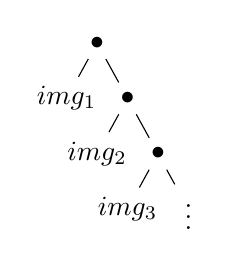
\begin{tikzpicture}[sibling distance=2.2em, level distance=2em]
  \node {\(\bullet\)}
    child { node {\(img_1\)} }
    child { node {\(\bullet\)}
      child { node {\(img_2\)}}
      child { node {\(\bullet\)}
        child { node {\(img_3\)}}
        child { node {\(\vdots\)}
    }}};
\end{tikzpicture}
\qquad
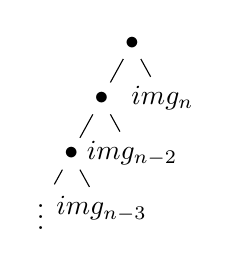
\begin{tikzpicture}[sibling distance=2.2em, level distance=2em]
  \node {\(\bullet\)}
    child { node {\(\bullet\)}
      child { node {\(\bullet\)}
        child {node {\(\vdots\)}}
        child {node {\(img_{n-3}\)}}}
      child { node {\(img_{n-2}\)}}
        }
    child { node {\(img_n\)} };
\end{tikzpicture}
\qquad
\begin{tikzpicture}[level distance=2em, level 3/.style={sibling distance=3em}, level 2/.style={sibling distance=2.5em}, level 1/.style={sibling distance=6em}]
  \usebeamercolor{example text}
  \node {\(\bullet\)}
  child { node[color=fg] {\(\bullet\)}
    child { node[color=fg] {\(\bullet\)}
      child {node[color=fg] {\texttt{zero}}}
      child {node[color=fg] {\(img_1\)}}}
    child { node[color=fg] {\(img_2\)}}
  }
  child { node[color=red] {\(\bullet\)}
    child { node[color=red] {\(img_3\)} }
    child { node[color=red] {\(\bullet\)}
      child { node[color=red] {\(img_4\)}}
      child { node[color=red] {\(\vdots\)}
      }}};
\end{tikzpicture}
\end{center}

  \note{
    Esses foram algums exemplos de de uso de Monoides, mas exemplos reducidos a
    pedacinhos de codigo. Poderiamos ter escrito esse codigo sem usar monoides,
    e nao seria grave. Mas vamos ver agora dois exemplos maiores, donde o monoide
    tem um rol muito mais importante na solucao.

    O primeiro eh um problema muito geral: precisamos combinar um monte de
    elementos a1, a2, etc. usando uma operacao que eh muito cara no CPU. Tem
    muitos exemplos disso, por exemplo, tem duas listas ordenadas, que quer
    fazer o merge e ficar com uma lista ordenada.

    \hrulefill

    Entao, como nos ajudams os monoides aqui? Se a operacao bullet fora um
    monoide, ou seja fora asociativa com identidade, sabemos que calcular
    qualquer um desses arbores dara o mesmo resultado. Cada um desses arbores
    equivale a colocar os parenteses de algum jeito diferente na expresao a1
    bullet a2 bullet a2 etc. e sabemos que como colocar os parenteses nao
    importa num monoide. Entao podemos por exemplo, escolher a arbore da
    dereita, evaluar as operacoes na sub-arbore vermelha num thread, e a verde
    num outro thread, e quando elas terminam, combinar os dois resultados. Mas
    tambem podemos fazer isso recursivamente e continuar dividindo a arbore e
    usar tantos threads como for melhor.

    De novo, isso so pode ser feito porque temos um monoide, uma operacao asociativa.

    O que temos que ter cuidado eh a ordem dos nodos, lembrando que nao todos os
    monoides sao commutativos, entao temos que combinar o resultado da arbore
    vermelha, a izquerda e a verde a direita cuando os combinamos com bullet.

    Esse eh um bom momento para pensar que acontece se escrebemos um monoide que
    nao cumple com as leis do monoide. O resultado estara incorreto! Cada vez
    que a gente correr o programa teremos um resultado diferente. Por isso,
    nunca escreba um monoide que nao satisfaiz as leis
  }
\end{frame}

\begin{frame}[fragile] \frametitle{LARGER USE CASES}
  \framesubtitle{Parallelization}

  \begin{block}{}
  \begin{lstlisting}
object Parallel {

  def mconcat[A:Monoid](as: Traversable[A]): A =
    ~\alt<1>{as.foldLeft(Monoid[A].zero)(\_ |+| \_)}{}\alt<2>{as.\alert{fold}(Monoid[A].zero)(\_ |+| \_)}{}\alt<3->{as.\usebeamercolor{structure}\textcolor{fg}{par}.\alert{fold}(Monoid[A].zero)(\_ |+| \_)}{}~
}
  \end{lstlisting}
  \end{block}

  \invisible<1>{
    \texttt{fold[A1 >: A](z: A1)(op: (A1, A1) => A1): A1}
    \vspace{2ex}

    \texttt{z}: a \alert{neutral} element for the fold operation;
    may be added to the result an arbitrary number of times, and \alert{must not change the result.}

    \texttt{op}: a binary operator that must be \alert{associative.}
    \begin{block}{}
      \centering
      \large \textbf{That's just a Monoid!}
    \end{block}
  }


  \note {
    Bom, como implementamos isso em paralelo? O unico que precisamos fazer
    eh reimplementar a funcao mconcat para correr em paralelo. Essa aqui e a
    implementacao que a gente tem. Como a transformamos em paralela?

    \hrulefill

    o primeiro que podemos fazer eh utilizar o metodo fold ao envez de foldLeft.
    Se olham a documentacao do scala, o metodo fold fala isso que esta ai
    embaixo. a operacao que passamos a fold deve ser asociativa e ter uma
    identidade. Ta vendo? eles nao falam em Monoide, mas isso eh exatamente um
    Monoide! E eles so podem implementar join para monoides pelos motivos que
    vimos.

    Join nao da garantia de em que ordem vai se fazer as evaluacoes, mas ainda
    nao eh paralela, so poderia correr em paralelo, eh a mesma coisa que
    foldLeft (um pouco menos geral no tipo), mas com limitacoes de que operacao
    e neutro pode se passar.

    \hrulefill

    Agora para convertir esse codigo em paralelo, so precissamos fazer uma coisa:
    convertir nosso traversable em um traversable paralelo. Pronto. Esse codigo
    vai correr em tantos threads como tenha disponivel o CPU.
  }
\end{frame}

% \begin{frame}[fragile] \frametitle{LARGER USE CASES}
%   \framesubtitle{Parallelization}
%   \begin{itemize}
%     \item You could have \emph{invented} the Monoid trying to write a parallel \texttt{fold}.
%     \item This is how you \emph{discover} the laws for an algebraic structure.
%     \item If you have a Monoid, you can \alert{fold it in parallel.}
%     \item But pay attention to the \alert{monoid laws!!!}
%     \item Huge performance win (in certain situations).
%     \item Base of several parallel and distributed frameworks.
%   \end{itemize}

% \end{frame}


\begin{frame} \frametitle{LARGER USE CASES}
  \framesubtitle{Incremental updates}
  \begin{block}{The Problem}
    For some measured magnitude (e.g. latency), \alert{compute and store mean and
    variance} Events arrive at high rate, \alert{millions per hour.}
  \end{block} \pause
  \begin{columns}[c]
    \column{0.6\textwidth}
      \begin{block}{Naive approach}
        \begin{itemize}
        \item Store all measurements,
        \item compute \(\mu, \sigma^2\) on demand, or
          precompute at certain interval.
        \end{itemize}
      \end{block}

    \column{0.3\textwidth}
  Too much \alert{space}, too much \alert{time}. \(\mathcal{O}(N)\)
  \end{columns}

  \pause

  \begin{columns}[c]
    \column{0.6\textwidth}
      \begin{block}{Unsound approach}
        \begin{itemize}
        \item Store previous \(\mu\) and \(\sigma^2\)
        \item on measurement average previous and current,
        \item store.
        \end{itemize}
      \end{block}

    \column{0.3\textwidth}
    Fast, low memory, \(\mathcal{O}(1)\) but \alert{incorrect}.
    \begin{align*}
      \mu[1,0,0] & = 1/3 \\
      \mu[\mu[1,0], 0] &= 1/4
    \end{align*}

  \end{columns}

  \note {
    Vamos agora para o ultimo problema que vamos estudar. Temos um sistema que
    mede alguma certa variable, por exemplo, o tempo que demora um request HTTP,
    ou cualquer outra coisa do tipo. Nosso sistema precisa calcular a media e
    variancia das medicoes. O que faz o problema mais complexo eh que as
    medicoes chegam muito rapidamente, vamos supor milhoes de medicoes por hora.
    Entao, chegam muitas medicoes, precisamos manter um computo da media e a
    variancia em algum tipo de banco de dados o store.

    \hrulefill

    A primeira ideia eh a mais simples. Cada vez que chega uma nova medicao,
    simplesmente guarda-la no banco de dados. Quando precisamos calcular a media
    ou variancia, carregamos todas as medicoes e calculamos. Se nao queremos
    esperar tanto quando precisamos a media, podemos precalcular ela a
    intervalos regulares e guardar. O problema eh que esse sistema eh de ordem N
    em espaco e tempo. Quantas mais medicoes temos mais lento fica, e com
    milhoes de medicoes por hora, nao vai funcionar.

    \hrulefill

    Uma ideia mais pratica seria ao envez de guardar no banco todas as medicoes,
    guardar so a media e a variancia. Depois, quando chega uma nova medicao, ou
    grupo de medicoes, calcular media e variancia e combinar com as anteriores.
    Esse algoritmo eh de ordem 1, nao precisso guardar as medicoes, mas para
    calcular medias, nao podo fazer a media das medias. Simplesmente a
    matematica nao funciona.

    Mas a ideia eh boa... combinar os resultados velhos com os novos... tem
    cheiro de monoide. So temos que arrumar a matematica.
  }
\end{frame}

\begin{frame} \frametitle{LARGER USE CASES}
  \framesubtitle{Incremental updates}
  \begin{block}{A better approach}
  \begin{itemize}
    \item Find a \alert{Monoid for mean/variance} of \(n\) samples.
    \item Serialize the Monoid to storage.
    \item Accumulate several (or 1) new measurements.
    \item \alert{Combine} the old and new results using the monoid.
    \item Store.
  \end{itemize}
  \end{block}

  \begin{block}{How is it better?}
  \begin{itemize}
    \item \alert{Exact} if we can find the right Monoid.
    \item \alert{\(\mathcal{O}(1)\) updates} (independent of sample size).
    \item Trade off freshness by scale.
  \end{itemize}
  \end{block}

  \note {
    Entao, como podemos fazer? O primeiro sera encontrar um monoide que consiga
    combinar os resultados de media e variancia anteriores com os novos. Depois,
    vamos acumulando medicoes, calculamos, e vamos guardando os resultados.
    Quando chegam novos resultados, o monoide sabe como combinar os velhos com
    os novos.

    Com esse algoritme vamos ter resultados exatos, se conseguimos escreber um
    monoide correto, as atualizacoes nao dependem da cantidad de dados. Outra
    ventagem eh que podemos decidir a cada quanto tempo combinar as medicoes,
    dependendo de que resolucao precisamos nos resultados. Podemos acumular
    medicoes por 1 segundo, ou 1 minuto, e so depois combinar com as velhas.
  }

\end{frame}

\begin{frame} \frametitle{LARGER USE CASES}
  \framesubtitle{Incremental updates}
  What to store?
  \begin{block}{Weighted average of the means}
    \[
    \begin{split}
      n\cdot \mu = \sum_{i=0}^{n-1} x_i \qquad  m\cdot \nu = \sum_{i=0}^{m-1} x_{i+n} \\
      \frac{1}{n+m} \sum_{i=0}^{n+m-1} x_i = \frac{n\mu + m\nu} {n+m}
    \end{split}
    \]
  \end{block}

  We need previous \alert{mean} and \alert{sample size.}

  Generalizing, to compute the nth-moment, we need to store n+1 values.

  \note {
    Entao, temos que desenhar nosso monoide. O que precisamos para conseguir
    combinar a media e variancia velhas com as novas? Essas equacoes ai, o que
    estao dizendo eh basicamente, que se eu tenho duas meias, que quero calcular
    a meia real dos dados, preciso calcular a meia mas usando pesos, o peso eh o
    tamanho de cada mostra. Entao multiplico a meia velha pelo seu tamanho e a
    nova tambem, somo e depois divido pela quantidade total de mostras.

    A formula da variancia eh mais complexa mas similar. Conclucao, para
    combinar meias e variancias, preciso guardar a meia, a variancia e o numero
    de mostras velhas.
  }
\end{frame}

\begin{frame}[fragile] \frametitle{LARGER USE CASES}
  \framesubtitle{Incremental updates}
  \begin{block}{A data type for mean and variance}
  \begin{lstlisting}
sealed abstract class MeanVar

final case object EmptyMeanVar extends MeanVar

final case class MeanVarV(
  m1: Double,
  m2: Double,
  n: Long) extends MeanVar
  \end{lstlisting}
  \end{block}

  \note {
    Entao, agora que sabemos o que guardar, vamos escreber um tipo. Meu tipo
    MeanVar aqui, eh um tipo soma. Pode ter duas formas: ou eh um Empty, no
    casso em que estou querendo computar a meia de 0 mostras, obviamente nao
    posso, entao a meia eh Empty. Ou posso calcular e nesse caso guardo 3
    valores: a meia m1, a variancia m2 e o tamanho da mostra n.

    Certo? Nada demais.

  }
\end{frame}

\begin{frame}[fragile] \frametitle{LARGER USE CASES}
  \framesubtitle{Incremental updates}
  \begin{block}{The Monoid}
  \begin{lstlisting}
val meanVarMonoid: Monoid[MeanVar] = new Monoid[MeanVar] {
  def zero: MeanVar = EmptyMeanVar

  def append(a: MeanVar, b: => MeanVar): MeanVar = (a, b) match {
    case (EmptyMeanVar, a) => a
    case (a, EmptyMeanVar) => a ~\pause~
    case (MeanVarV(m1a, m2a, na), MeanVarV(m1b, m2b, nb)) => {
      val nt = na + nb
      val delta = m1b - m1a
      MeanVarV(~\alert{(na * m1a + nb * m1b ) / nt}~,
                m2a + m2b + delta * delta * na * nb / nt,
                ~\alert{nt}~)
    }
  }
}
  \end{lstlisting}
  \end{block}

  \note {
    Agora vamos a escreber o monoide para MeanVar. A identidade que seria? Tem
    que ser um MeanVar que nao mude os outros MeanVars quando se combina, entao
    vai ser o EmptyMeanVar. Podem pensar que estaria combinando uma mostra com
    uma mostra vazia, isso nao vai alterar a mostra.

    Otimo. O append agora, tenho dois MeanVar e perciso devolver um outro. Se um
    dos dois eh o EmptyMeanVar, nao preciso fazer nada, eh a identidade, entao
    simplesmente devolvo o outro MeanVar.

    E para o caso em que realmente preciso combinar dois MeanVars com dados, eh
    so aplicar a formula que vimos antes. Se olham a parte em vermelho, estou
    aplicando a formula, o promedio pesado pelo tamanho da mostra. A formula da
    variancia eh um pouco mais complicada, mas nada demais.

    Pronto, temos um monoide que sabe combinar medias e variancias.
  }
\end{frame}

\begin{frame}[fragile] \frametitle{LARGER USE CASES}
  \framesubtitle{Incremental updates}
  \begin{block}{Utility functions: creating \texttt{MeanVars}}
  \begin{lstlisting}
object MeanVar {

  def singleton(x: Double): MeanVar = MeanVarV(x, 0, 1)

  def sample(xs: Traversable[Double]): MeanVar = ~\pause~
    foldMap(xs, singleton)
}
  \end{lstlisting}
  \end{block}

  \note {
    So faltaria agora escreber umas funcoes para poder criar esses objetos
    MeanVar, vamos coloca-las no objeto companion

    Primeiro uma funcao chamada singleton para crear um MeanVar quando a mostra tem um unico
    valor. Se quero calcular a media de uma mostra com um unico ponto,
    obviamente a media eh o valor do ponto, a variancia cero, e o numero de
    mostras 1.

    Agora vamos ao caso mais interessante, calcular o MeanVar para uma mostra.
    Como podemos fazer? [esperar]

    \hrulefill

    Bom, tem muitas formas possivels. Mas a mais
    facil eh, convertir a cada ponto em um MeanVar com 1 dato so, e depois
    combinar todos eles com o monoide. Como fazo isso? Com nossa querida
    foldMap. Mapeio todos os pontos aplicando a funcao singleton, e depois o
    monoide vai combinar todos eles.

    E pronto, temos todo o que precisavamos.
  }
\end{frame}

% \begin{frame}[fragile] \frametitle{LARGER USE CASES}
%   \framesubtitle{Incremental updates}
%   \begin{block}{Utility functions: extracting from \texttt{MeanVars}}
%   \begin{lstlisting}
% object MeanVar {
%   def sampleSize: MeanVar => Long = {
%     case MeanVarV(_, _, n) => n
%     case _ => 0
%   }
%   def mean: MeanVar => Option[Double] = {
%     case MeanVarV(m1, _, _) => Some(m1)
%     case _ => None
%   }
%   def variance: MeanVar => Option[Double] = {
%     case MeanVarV(_, _, 1) => Some(0)
%     case MeanVarV(_, m2, n) => Some(m2/(n - 1.0))
%     case _ => None
%   }
% }
%   \end{lstlisting}
%   \end{block}
% \end{frame}

\begin{frame}[fragile] \frametitle{LARGER USE CASES}
  \framesubtitle{Incremental updates}
  \begin{block}{Updating the statistics (pseudocode)}
  \begin{lstlisting}
     // Define a time resolution (accumulate for 1sec? 100ms?)
     val newSample: Vector[Double] = getNewMeasurements(...)

     // Compute mean/var of the new data (incremental work)
     val newStats: MeanVar = MeanVar.sample(newSample)

     // This is an O(1) op
     // In our example this loads 3 numbers,
     // doesn't matter how many samples we have processed before
     val oldStats: MeanVar = loadStats(...)

     // Another O(1) operation
     storeStats(oldStats |+| newStats)
  \end{lstlisting}
  \end{block}

  \note {
    So resta escreber o algoritmo completo, que vamos fazer em pseudocodigo.

    Tenho uma forma de obter as medicoes novas, chamadas aqui de newSample. Isso
    pode ser um callback toda vez que tem uma medicao nova, o pode esperar ate
    acumular uma certa quantidade de medicoes, ou pode esperar ate acumular por
    certo tempo.

    Depois, usando nossa funcao sample podemos convertir essas medicoes em um
    MeanVar, chamado aqui de newStats.

    Depois, vou no banco de dados e obtenho o MeanVar antigo. Percebam que isso
    eh uma operacao muito simples, so preciso trazer 3 numeros do banco.

    Finalmente, uso o monoide de MeanVar para combinar a velha com a nova, e
    guardo no banco de dados.

  }
\end{frame}


\begin{frame} \frametitle{LARGER USE CASES}
  \framesubtitle{Incremental updates}
  \begin{block}{Some details}{}
  \begin{itemize}
    \item We never wrote the alg. to compute mean/var, only to
    \item Extensible to higher momenta.
    \item Extensible to approximate histograms and other fun stuff.
      combine them.
    \item Didn't we say \texttt{Double} under \texttt{(+)} is not a Monoid?
  \end{itemize}
  \end{block}
  % \begin{block}{Take-home quiz}
  %   \begin{itemize}
  %   \item How can we do rolling averages? We would need to \emph{delete} the older
  %   accumulated data.
  %   \item Write two different Monoids for \texttt{Map[K, V]}. Do you need to
  %     impose restrictions on \texttt{V}?
  %   \end{itemize}
  % \end{block}

  \note {
    Algums detalhes.

    Ese mecanismo pode ser extendido para calcular coisas mais interessantes que
    media e variancia, pode calcular kurtosis skewness e de  fato cualquer
    momento da distribuicao. De fato pode se calcular em aproximacao outras
    coisas tambem usando um monoide, como histogramas por exemplo.

    Eh interessante ver que nunca escribimos o algoritmo de media ou variancia,
    so explicamos como combinar duas medias e duas variancias. Com isso eh
    suficiente para que o monoide faza todo o trabalho. Meio magico neh?

    E finalmente ... lembra que falei que os doubles com a soma nao erao um
    monoid? como poderia ser isso que tem um monte de artimetica de monoide?
    Bom, na verdade nao eh, mas para numeros razoavels a aproximacao eh
    suficentemente boa.

  }
\end{frame}

\begin{frame} \frametitle{CONCLUSIONS}
  \begin{itemize}
    \item You could have \emph{invented} the Monoid trying to write incremental
      updates or trying to parallelize your code.
    \item \emph{Discover} the laws for an algebraic structure.
    \item Write only \alert{lawful} Monoids.
    \item \alert{USE THE MONOID}. They are everywhere.
    \item Don't be afraid of other algebraic structures (Functor, Monad).
      \item \alert{Learn how to abstract}, if possible learn from the best.
  \end{itemize}
  % \begin{block}{Take-home quiz}
  %   \begin{itemize}
  %   \item How can we do rolling averages? We would need to \emph{delete} the older
  %   accumulated data.
  %   \item Write two different Monoids for \texttt{Map[K, V]}. Do you need to
  %     impose restrictions on \texttt{V}?
  %   \end{itemize}
  % \end{block}

  \note {
    Conclusoes.

    Esses dois ultimos exemplos, a parallelizacao e update incremental, sao boms
    exemplos de como voce poderia ter inventado o monoide. Tentando escreber o
    algoritmo paralelo, voce tevese descoberto que ia funcionar so, se a
    operacao eh asociativa, e so se a identidade se pode combinar sem
    consequencias. Tevesse chamado isso de algum outro jeito, por exemplo como a
    documentacao de scala faz, mas ... voce tevera reinventado o monoide.

    Lembre o que acontece se seus monoides nao cumplem com as leis do monoide:
    resultado incorreto, nunca faza isso.

    No contrario, se voce ja sabe do monoide, recomendo que voce pense neles
    quando esta tentando resolver um problema, vai perceber que ajuda muito a
    resolver problemas e para abstraer suas solucoes.

    Finalmente, aprenda abstracao, aprenda de onde puder, mas se um dia tiver
    vontades, da uma leida em algum tema de matematica abstrata, vais se
    surprender com quanto se parece com programacao.

  }
\end{frame}

\subsection*{References}
\begin{frame} \frametitle{REFERENCES}
  \begin{columns}[c]
    \column{0.7\textwidth}
      \begin{itemize}

        \item This talk: slides, all the \alert{code and many tests} \\
          \href{https://github.com/paraseba/scaladores-may-2018}{\underline{https://github.com/paraseba/scaladores-may-2018}} % fixme

        \item \textit{Functional Programming in Scala.}\\ Paul Chiusano \& Runar Bjarnason

        \item \textit{Why Functional Programming Matters} \\
          John Hughes.

        \item \textit{Computing skewness and kurtosis in one pass.} \\
          {\footnotesize \href{https://www.johndcook.com/blog/skewness\_kurtosis/}{\underline{https://www.johndcook.com/blog/skewness\_kurtosis/}}}

        \item Scalaz library \\
          {\href{https://github.com/scalaz/scalaz}{\underline{https://github.com/scalaz/scalaz}}}
      \end{itemize}

    \column{0.3\textwidth}

    \begin{figure}
        \vspace{10ex}
        \centering
        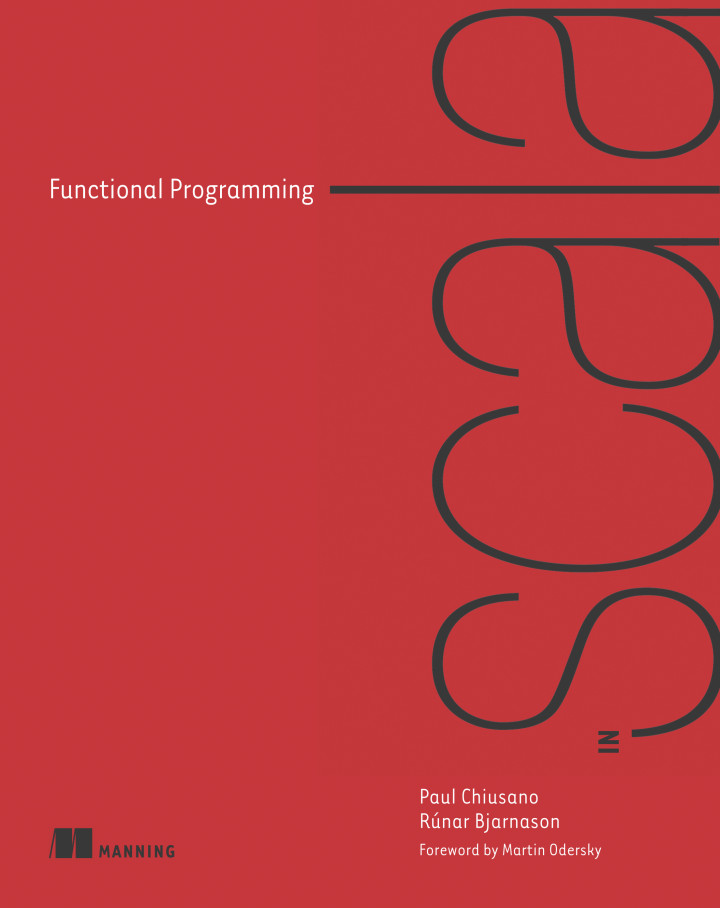
\includegraphics[width=\textwidth]{functional-programming-in-scala.png}
    \end{figure}
  \end{columns}

  \note {
    Se voces querem ver os slides, ou o codigo que tem testes  poder achar no
    meu github

    Se voces querem aprender mais, recomendo muito o livro Functional
    Programming in Scala. Eh uma des melhores introducoes a PF que ja vi, em
    cualquer linguagem.

    Se querem uma coisa mais basica e curta de programacao funcional, em haskell
    ao envez de scala, o paper why functional programming matters eh
    maravilhoso, recomendo ler tudo ano.

    Se querem brincar com PF em scala, tem muitas bibliotecas muito boas. Mas
    para nombra uma, podem olhar scalaz, que eh muito completa. A documentacao
    deixa bastante a desejar mas, acompanhando com o livro e trabalho, pode ser feito.

  }
\end{frame}

\section{Monoids in Design [next session]}

\begin{frame}{Monoids in Design (ToDo)}
\end{frame}


% \begin{frame}{ToDo / Fixme}
%   \begin{itemize}
%     \item grammarly
%     \item topic for design session: aggregations (a la beautiful folds)
%   \end{itemize}
% \end{frame}

\end{document}